\documentclass[12pt]{Report}
\usepackage{graphicx}
\usepackage{listings}

\usepackage{verbatim} 

\begin{document}
\title{Assignment 3 : CS 751 }
\author{HARISH}

\maketitle

\section{Part 1}

\paragraph{For the text you saved for the 10000 URIs from A1, Q2:
Use the “boilerpipe” software to remove the HTML templates from all HTML pages (document how many pages link from the tweets were non-HTML and had to be skipped)
https://code.google.com/p/boilerpipe/ 
WSDM 2010 paper: http://www.l3s.de/~kohlschuetter/boilerplate/
For how many of the 10000 URIs was boilerpipe successful? 
Compare the total words, unique words, and byte sizes before and after use of boilerpipe
For what classes of pages was it successful?  
For what classes of pages was it unsuccessful?
Provide examples of both successful and unsuccessful removals and discuss at length. \\ \\
}

I have used jusText library to remove HTML templates. It removes headers, footers and navigation links from the page.
I have written a code in python named "htmlnonhtml.py" which removes boilerplate content from the links.\\

Total words before removing boiler content plate is 64221898 and after removing boiler content plate is 91666 .
Total unique words before removing boiler content plate is 2979715. Total unique words after removing boiler content is "19418". \\

Only 6100 links were unique , out of this 1496 are successful . Most of them are non-HTML skipped because of non content , Images on links , 404, 302 errors etc.

The size of the file before removing boiler content is "573,080 KB" and after removing boiler content is "553 KB".\\
 
 
jusText was unsuccessful for pages that did not follow HTML standards. Pages which are not properly organized .

Below figure1 represents unsuccessful class of page.\\


\subsubsection{Unsuccessful Class of Page}
\begin{figure}[ht]    
    \begin{center}
        
\includegraphics[scale=0.60]{unsuccessful.png}
        \caption{Unsuccessful  Class of Page}
        \label{}
    \end{center}
\end{figure}
\newpage


jusText was successful for pages that followed HTML standards. Pages which are properly organized .\\

Below figure2 represents successful class of Page.

\subsubsection{successful Class of Page}
\begin{figure}[ht]    
    \begin{center}
        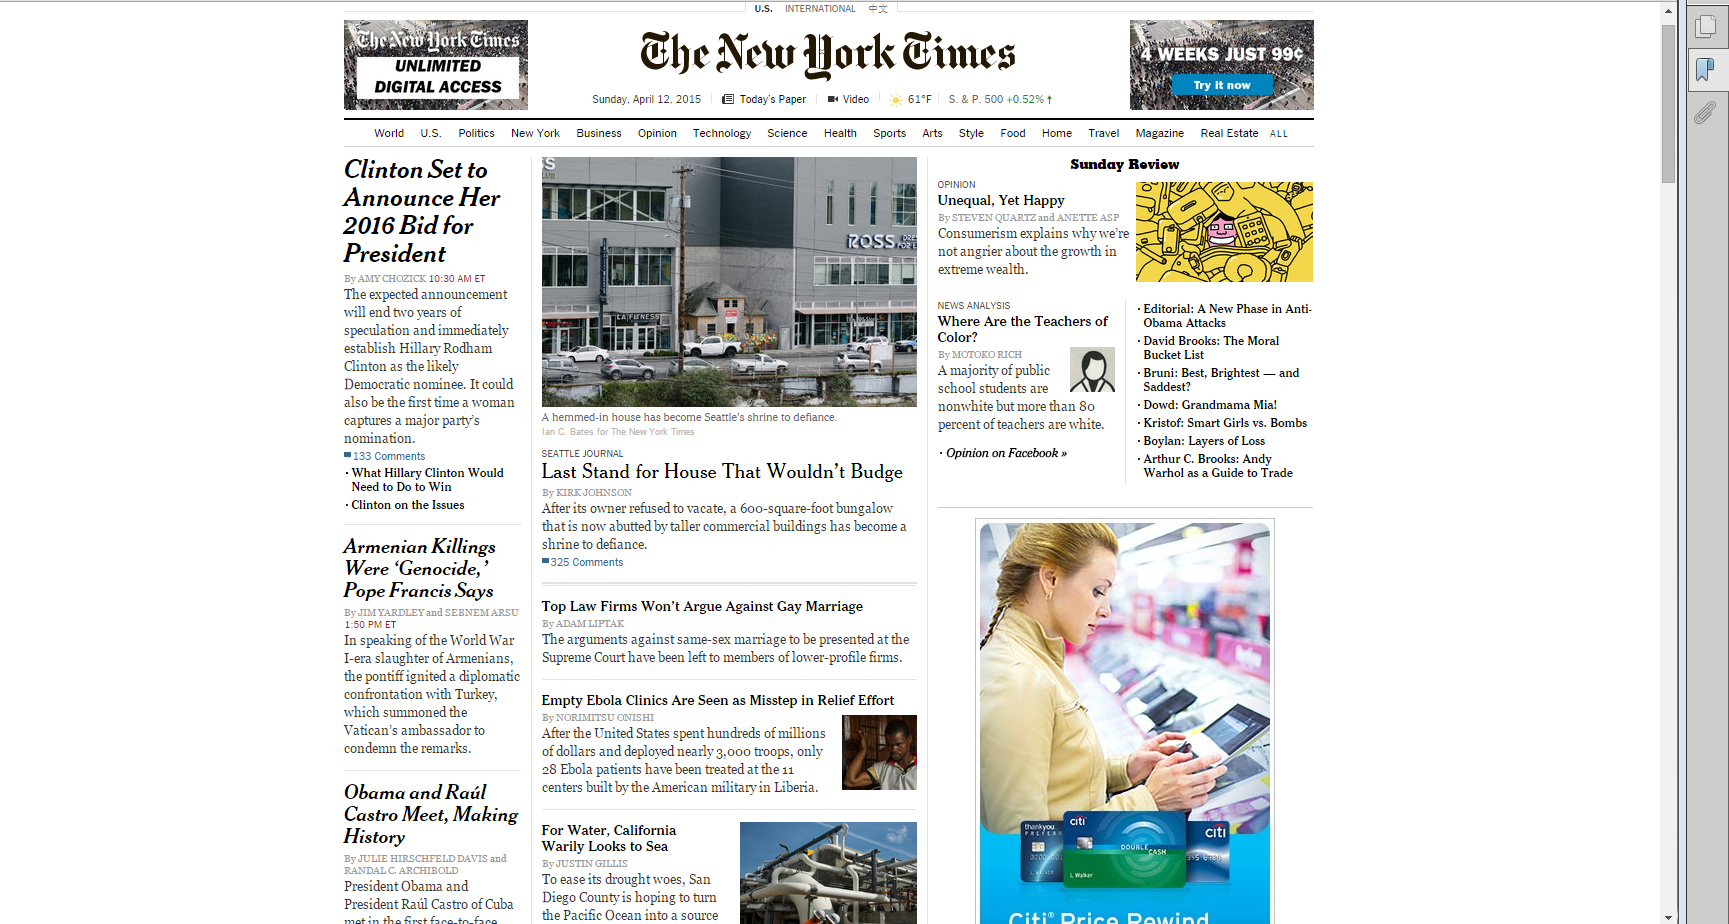
\includegraphics[scale=0.60]{SuccessfulPage.png}
        \caption{successful  Class of Page}
        \label{}
    \end{center}
\end{figure}
\newpage


\paragraph{Collection1: Extract all the unique terms and their frequency from the 10000 files*
Collection2: Extract all the unique terms and their frequency of the 10000 files* after running boilerpipe
Construct a table with the top 50 terms from each collection. 
Find a common stop word list.  How many of the 50 terms are on that stop word list?
For both collections, construct a graph with the x-axis as word rank, and y-axis as word frequency.  
Do either follow a Zipf distribution? Support your answer.
 }


I have extracted extracted all the unique terms and their frequency from the 10000 files. This is done using "getwordcount.py" . All the words before applying boliler pipe  are stored in "wordcountbeforeboiler.txt".\\

Also , i have extracted all the unique terms and their frequency and stored in "wordcountafterboiler.txt".\\

I have also extracted top 50 words with their frequency into "fiftywordcountbeforeboiler.txt" before applying boiler pipe .This file "fiftywordcountafterboiler.txt" contains top 50 words with their frequency after applying boilerpipe.



Below figure 3 has  top 50 words with their frequencies before applying boiler pipe.

Below figure 3 has top 50 words with their frequencies after applying boiler pipe.


41 words  are found common from text file from the stop word list which I got from internet. 

14  words are found common from words extracted from html file .

\newpage
\begin{table}
\caption{Rank, word and frequency using jusText }
\begin{center}
  \begin{tabular}{ c | c | c }
    \hline
    RANK & WORD & FREQUENCY \\ \hline
1 & the  &  4444 \\ \hline
2 & and & 3037 \\ \hline
3 & to & 2753 \\ \hline
4 & of & 2015 \\ \hline
5 & a  & 1862 \\ \hline
6 & in & 1653 \\ \hline
7 & you & 1330 \\ \hline
8 & is & 1037 \\ \hline
9 & for  & 968 \\ \hline
10 & are  & 847 \\ \hline
11 & that & 764 \\ \hline
12 & on &  754 \\ \hline
13 & with  &  699 \\ \hline
14 & this & 693 \\ \hline
15 & it & 569 \\ \hline
16 & or & 562 \\ \hline
17 & i & 555 \\ \hline
18 & your  & 554 \\ \hline
19 & be  & 534 \\ \hline
20 & by & 525 \\ \hline
21 & if &   504 \\ \hline
22 & from & 495 \\ \hline
23 & as   & 494 \\ \hline
24 & have & 459 \\ \hline
25 & we & 451 \\ \hline
26 & will & 413 \\ \hline
27 & at & 384 \\ \hline
28 & not & 382 \\ \hline
29 & our &  354 \\ \hline
30 & an  & 342 \\ \hline
31 & more & 325 \\ \hline
32 & new & 319 \\ \hline
33 & can &  314 \\ \hline
34 & all & 302 \\ \hline
35 & was & 282 \\ \hline
36 & but &  260 \\ \hline
37 & he & 232 \\ \hline
38 & their & 219 \\ \hline
39 & about & 213 \\ \hline
40 & my & 211 \\ \hline
41 & they & 207 \\ \hline
42 & has & 194 \\ \hline
43 & his & 190 \\ \hline
44 & so & 186 \\ \hline
45 & do & 183 \\ \hline
46 & any & 181 \\ \hline
47 & one& 179 \\ \hline
48 & when & 158 \\ \hline
49 & has & 156 \\ \hline
50 & any &  152 \\ \hline
    \hline
  \end{tabular}
  \label{table:textFiles}
\end{center}
\end{table} 

\begin{table}
\caption{ Top 50 terms extracted from HTML files}
\begin{center}
\begin{tabular}{ c | c | c }
 \hline
 RANK & TERM & FREQUENCY \\ \hline
1 &div &5921\\ \hline
2 &= &3933\\ \hline
3 &the &3711\\ \hline
4 &<a &3511\\ \hline
5 &to &3408\\ \hline
6 &and &3390\\ \hline
7 &a &3270\\ \hline
8 &of &3110\\ \hline
9 & \{&3032\\ \hline
10 &\textless li \textgreater \textless a &2913\\ \hline
11 &\textless span &2878\\ \hline
12 &\textless /div \textgreater &2773\\ \hline
13 &in &2683\\ \hline
14 &\{. &2583\\ \hline
15 &for &2480\\ \hline
16 &- &2310\\ \hline
17 & \textless li &2237\\ \hline
18 &at &2137\\ \hline
19 &var &2031\\ \hline
20 &point:false, &1997\\ \hline
21 &on &1896\\ \hline
22 &+ &1793\\ \hline
23 &\textless /div \textgreater &1633\\ \hline
24 &is &1489\\ \hline
25 & target='self' & 1211\\ \hline
26 &? &1031\\ \hline
27 &position:'left'\}, &937\\ \hline
28 &yous &820\\ \hline
29 &your &708\\ \hline
30 & \textless /li \textgreater&681\\ \hline
31 &class="user-in" &608\\ \hline
32 &with &585\\ \hline
33 &I &565\\ \hline
34 &user &550\\ \hline
35 &target='' &520\\ \hline
36 &\&amp; &482\\ \hline
37 &2014 &472\\ \hline
38 & \textless /a \textgreater &460\\ \hline
39 &December &452\\ \hline
40 &0 &400\\ \hline
41 &rel='fll' &368\\ \hline
42 &\textless img &355\\ \hline
43 &onclick="return &352\\ \hline
44 &if &350\\ \hline
45 & follow:false,&348\\ \hline
46 &class="hight" &337\\ \hline
47 &type="hidden" &333\\ \hline
48 &The &322\\ \hline
49 &alt &306\\ \hline
50&class="high &296\\ \hline
    \hline
  \end{tabular}
\end{center}
\label{table:htmlFiles}
\end{table}

I have plotted the top 50 words frequency distribution using RStudio for the words which i have extracted brfore applying boiler plate and after applying boiler plate.\\
The script "frequencyrankComparsion.R" exports the frequency distribution graph for words after applying boiler plate.It is shown in Figure 3. \\

 The script "htmlData.R" exports the frequency distribution graph for words before applying boiler plate.It is shown in Figure 4.
 
 Figure3,4 doesn't follow zipf distribution. Most frequent word  that occurred did not approximately equal to twice as often as the second most frequent word ,three times as often as the third most frequent word and so on.\\




\newpage
\subsubsection{ Frequency Distribution of top 50 words before boiler plate}
\begin{figure}[ht]    
    \begin{center}
        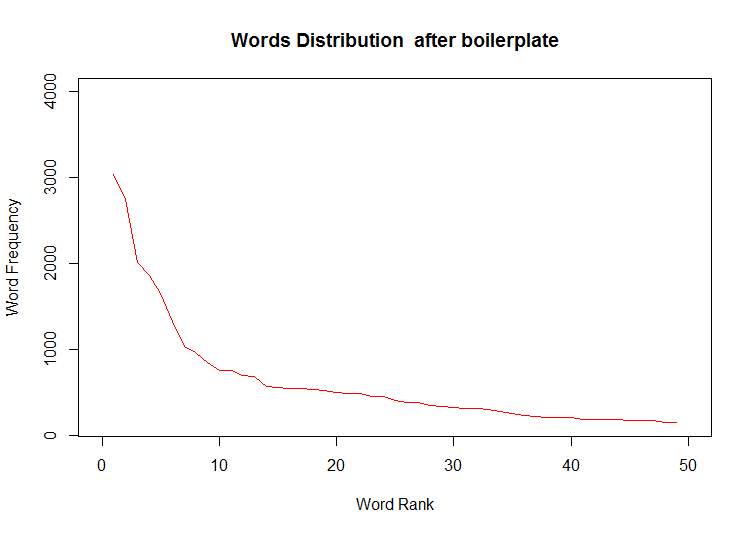
\includegraphics[scale=0.60]{afterboilerplate.png}
        \caption{}
        \label{}
    \end{center}
\end{figure}

\newpage
\subsubsection{ Frequency Distribution of top 50 words after boiler plate}
\begin{figure}[ht]    
    \begin{center}
        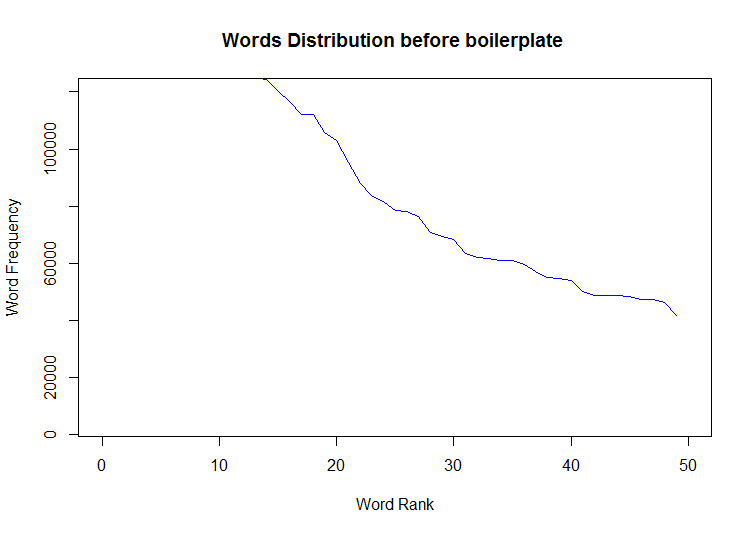
\includegraphics[scale=0.60]{beforeboilerplate.png}
        \caption{}
        \label{}
    \end{center}
\end{figure}
 
\end{document}



